%----------------------------------------------------------------------------------------
%       PACKAGES AND THEMES
%
% docs: https://en.wikibooks.org/wiki/LaTeX/Presentations#Introductory_example
%----------------------------------------------------------------------------------------


\documentclass{beamer}

\mode<presentation> {

% The Beamer class comes with a number of default slide themes
% which change the colors and layouts of slides. Below this is a list
% of all the themes, uncomment each in turn to see what they look like.

%\usetheme{default}
%\usetheme{AnnArbor}
%\usetheme{Antibes}
%\usetheme{Bergen}
%\usetheme{Berkeley}
\usetheme{Berlin}
%\usetheme{Boadilla}
%\usetheme{CambridgeUS}
%\usetheme{Copenhagen}
%\usetheme{Darmstadt}
%\usetheme{Dresden}
%\usetheme{Frankfurt}
%\usetheme{Goettingen}
%\usetheme{Hannover}
%\usetheme{Ilmenau}
%\usetheme{JuanLesPins}
%\usetheme{Luebeck}
%\usetheme{Madrid}
%\usetheme{Malmoe}
%\usetheme{Marburg}
%\usetheme{Montpellier}
%\usetheme{PaloAlto}
%\usetheme{Pittsburgh}
%\usetheme{Rochester}
%\usetheme{Singapore}
%\usetheme{Szeged}
%\usetheme{Warsaw}

% As well as themes, the Beamer class has a number of color themes
% for any slide theme. Uncomment each of these in turn to see how it
% changes the colors of your current slide theme.

%\usecolortheme{albatross}
%\usecolortheme{beaver}
%\usecolortheme{beetle}
\usecolortheme{crane}
%\usecolortheme{dolphin}
%\usecolortheme{dove}
%\usecolortheme{fly}
%\usecolortheme{lily}
%\usecolortheme{orchid}
%\usecolortheme{rose}
%\usecolortheme{seagull}
%\usecolortheme{seahorse}
%\usecolortheme{whale}
%\usecolortheme{wolverine}

%\setbeamertemplate{footline} % To remove the footer line in all slides uncomment this line
%\setbeamertemplate{footline}[page number] % To replace the footer line in all slides with a simple slide count uncomment this line

%\setbeamertemplate{navigation symbols}{} % To remove the navigation symbols from the bottom of all slides uncomment this line
}

%\usepackage[german]{babel}
\usepackage[latin1]{inputenc}
\usepackage{alltt}
\usepackage{beamerthemesplit}

\usepackage{graphicx} % Allows including images
\usepackage{booktabs} % Allows the use of \toprule, \midrule and \bottomrule in tables

\usepackage{color}
\usepackage{listings}
\lstset{
  %basicstyle=\ttfamily\bfseries,
  basicstyle=\ttfamily\footnotesize,
  commentstyle=\color{red}\itshape,
  stringstyle=\color{green},
  showstringspaces=false,
  keywordstyle=\color{blue}\bfseries,
  numberstyle=\ttfamily\tiny,
  frame=single,
  numbers=left,
  numbersep=1em,
  xleftmargin=2em,
  language=Python,
  breaklines=true,
  breakatwhitespace=true,
  postbreak=\hbox{$\hookrightarrow$ },
  showstringspaces=false,
  tabsize=2
}



%% Title Page

\title{Birdhouse Web Processing Services}
\subtitle{EGI Workshop: Design your e-Infrastructure}
\author{
Carsten Ehbrecht\\
\medskip
{\scriptsize \url{ehbrecht@dkrz.de}}
}
\institute{German Climate Computing Center (DKRZ)}
\date{April 2016}
\subject{Climate Science, Web Processing Service}

% page numbers
%\insertframenumber

% don't count title page
%\addtocounter{framenumber}{-1}


%------------------------------------------------

\begin{document}

%------------------------------------------------

  \begin{frame}[plain]
    \titlepage
  \end{frame}

%------------------------------------------------

  %\AtBeginSection[]
  \AtBeginSection[]{\frame{\frametitle{Overview}\tableofcontents[current]}}
  {
    \begin{frame} % shrink
      \frametitle{Outline}
      \tableofcontents[subsectionstyle=hide/hide]
    \end{frame}
  }

%------------------------------------------------

  \section{Use Case}

  % \begin{frame}
  %   \frametitle{Web Processing Service}
  %   A web service interface to standardize the way that algorithms are made available on the Internet
  %   \begin{figure}
  %     \includegraphics[width=7cm]{images/Wps.png}
  %   \end{figure}
  % \end{frame}

%------------------------------------------------

  \begin{frame}
    \frametitle{WPS Use Case}
    WPS: A web service interface to standardize the way that algorithms are made available on the Internet
    \begin{figure}
      \includegraphics[width=11.5cm]{images/WpsUseCase.png}
    \end{figure}
  \end{frame}

%------------------------------------------------

  \begin{frame}
    \frametitle{Example: Ensemble Robustness Process}
    \begin{figure}
      \includegraphics[width=11.5cm]{images/wps-ensemble-robustness.png}
    \end{figure}
  \end{frame}

%------------------------------------------------

  \begin{frame}
    \frametitle{Birdhouse Overview}
    \begin{figure}
      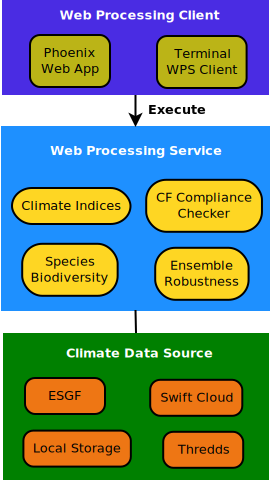
\includegraphics[width=4cm]{images/birdhouse-simple.png}
    \end{figure}
  \end{frame}

%------------------------------------------------

  \section{Question and Answers}

  \begin{frame}
    \frametitle{Background}
    \begin{itemize}
      \item Who is the community the use case belongs to?
      \item What's the timeline for development, tests and large-scale operation?
      \item What's your role in the use case? Any experience/link to EGI? 
    \end{itemize}
  \end{frame}

%------------------------------------------------

   \begin{frame}
    \frametitle{Users}
    \begin{itemize}
      \item Who will be the users of the planned community-specific e-infrastructure? How many of them?
      \item How will the users interact with the system - Show this on a system architecture diagram
      \item Who and how would validate the system? 
    \end{itemize}
  \end{frame}

%------------------------------------------------

   \begin{frame}
    \frametitle{Status}
    \begin{itemize}
      \item Which components/services already exist in your architecture?
      \item Which components/services are under development (and by who)?
      \item Which components/services do you expect to get from EGI? 
    \end{itemize}
  \end{frame}

%------------------------------------------------

  \begin{frame}
    \frametitle{Birdhouse Components}
    \begin{figure}
      \includegraphics[width=10cm]{images/birdhouse-components.png}
    \end{figure}
  \end{frame}

%------------------------------------------------

  \begin{frame}
    \frametitle{Copernicus}
    \begin{figure}
      \includegraphics[width=8cm]{images/wps-copernicus-use-case.png}
    \end{figure}
  \end{frame}

%------------------------------------------------

  \begin{frame}
    \frametitle{Twitcher}
    \begin{figure}
      \includegraphics[width=10cm]{images/twitcher-overview.png}
    \end{figure}
  \end{frame}

%------------------------------------------------

   \begin{frame}
    \frametitle{Plans for today}
    \begin{itemize}
      \item What questions would you like to get answered today?
      \item What issues you would like to solve today?
      \item Other outcomes that you would like to get out from the workshop? 
    \end{itemize}
  \end{frame}

%------------------------------------------------

  \appendix

  \section{Appendix}
  
   \begin{frame}[allowframebreaks]
    \frametitle<presentation>{Further Reading}    
    \begin{thebibliography}{10}    
      \beamertemplatearticlebibitems
    \bibitem{birdhouse}
      Birdhouse
      \newblock \url{http://bird-house.github.io/}
    \bibitem{buildout}
      Buildout
      \newblock \url{http://www.buildout.org/}
    \bibitem{anaconda}
      Anaconda
      \newblock \url{https://www.continuum.io/why-anaconda}
    \bibitem{foos4g-ebrahim}
      Evaluation of WPS Frameworks
      \newblock \url{http://www.slideshare.net/mepa1363/foss4g-ebrahim}
    \bibitem{wps-cct}
      Web Processing Service
      \newblock http://www.slideshare.net/GasperiJerome/20130530-web-processing-service-cct-cloud-toulouse-29423710
   
    \end{thebibliography}
    
  \end{frame}
  
%------------------------------------------------

  \begin{frame}
    \Huge{\centerline{The End}}
  \end{frame}

%------------------------------------------------

\end{document}
